\chapter{Экспериментальные исследования системы}
\label{ch:experiment}

Как уже было сказано в предыдущем разделе~\ref{ch:zemax}, в качестве приёмника был выбран фотодиод FDGA05. Рассчитаем пропускную способность $f_{BW}$ этого фотодиода по данным производителя~\cite{PDThorlabs}:

\begin{equation}
    f_{BW} = \frac{1}{2\pi R_L C_j},
\end{equation}

где $R_L = 50$ Ом \--- сопротивление нагрузки, $C_j = 10$ пФ $= 10^{-11}$ Ф \--- ёмкость фотодиода. Тогда $f_{BW} = 3.1831 \cdot 10^8~\text{Гц} = 318.31~\text{МГц}$.

Экспериментально подтвердим это значение. Для этого соберём экспериментальную установку, состоящую из фотодиода FDGA05~\cite{PDThorlabs} и лазерного диода FPL1055T~\cite{LDThorlabs}. Оба компоненты распаяны на платы для подключения к векторному анализатору цепей Rohde & Schwarz ZVA 40 через SMA разъем (собранная установка аналогично установке представлена на рисунке~\ref{fig:experiment_setup_photo}: на ней показаны лазерный диод FPL1055T слева и фотодиод, использованный в работе~\cite{Kozyreva2019}).

\begin{figure}[!h]
    \centering
    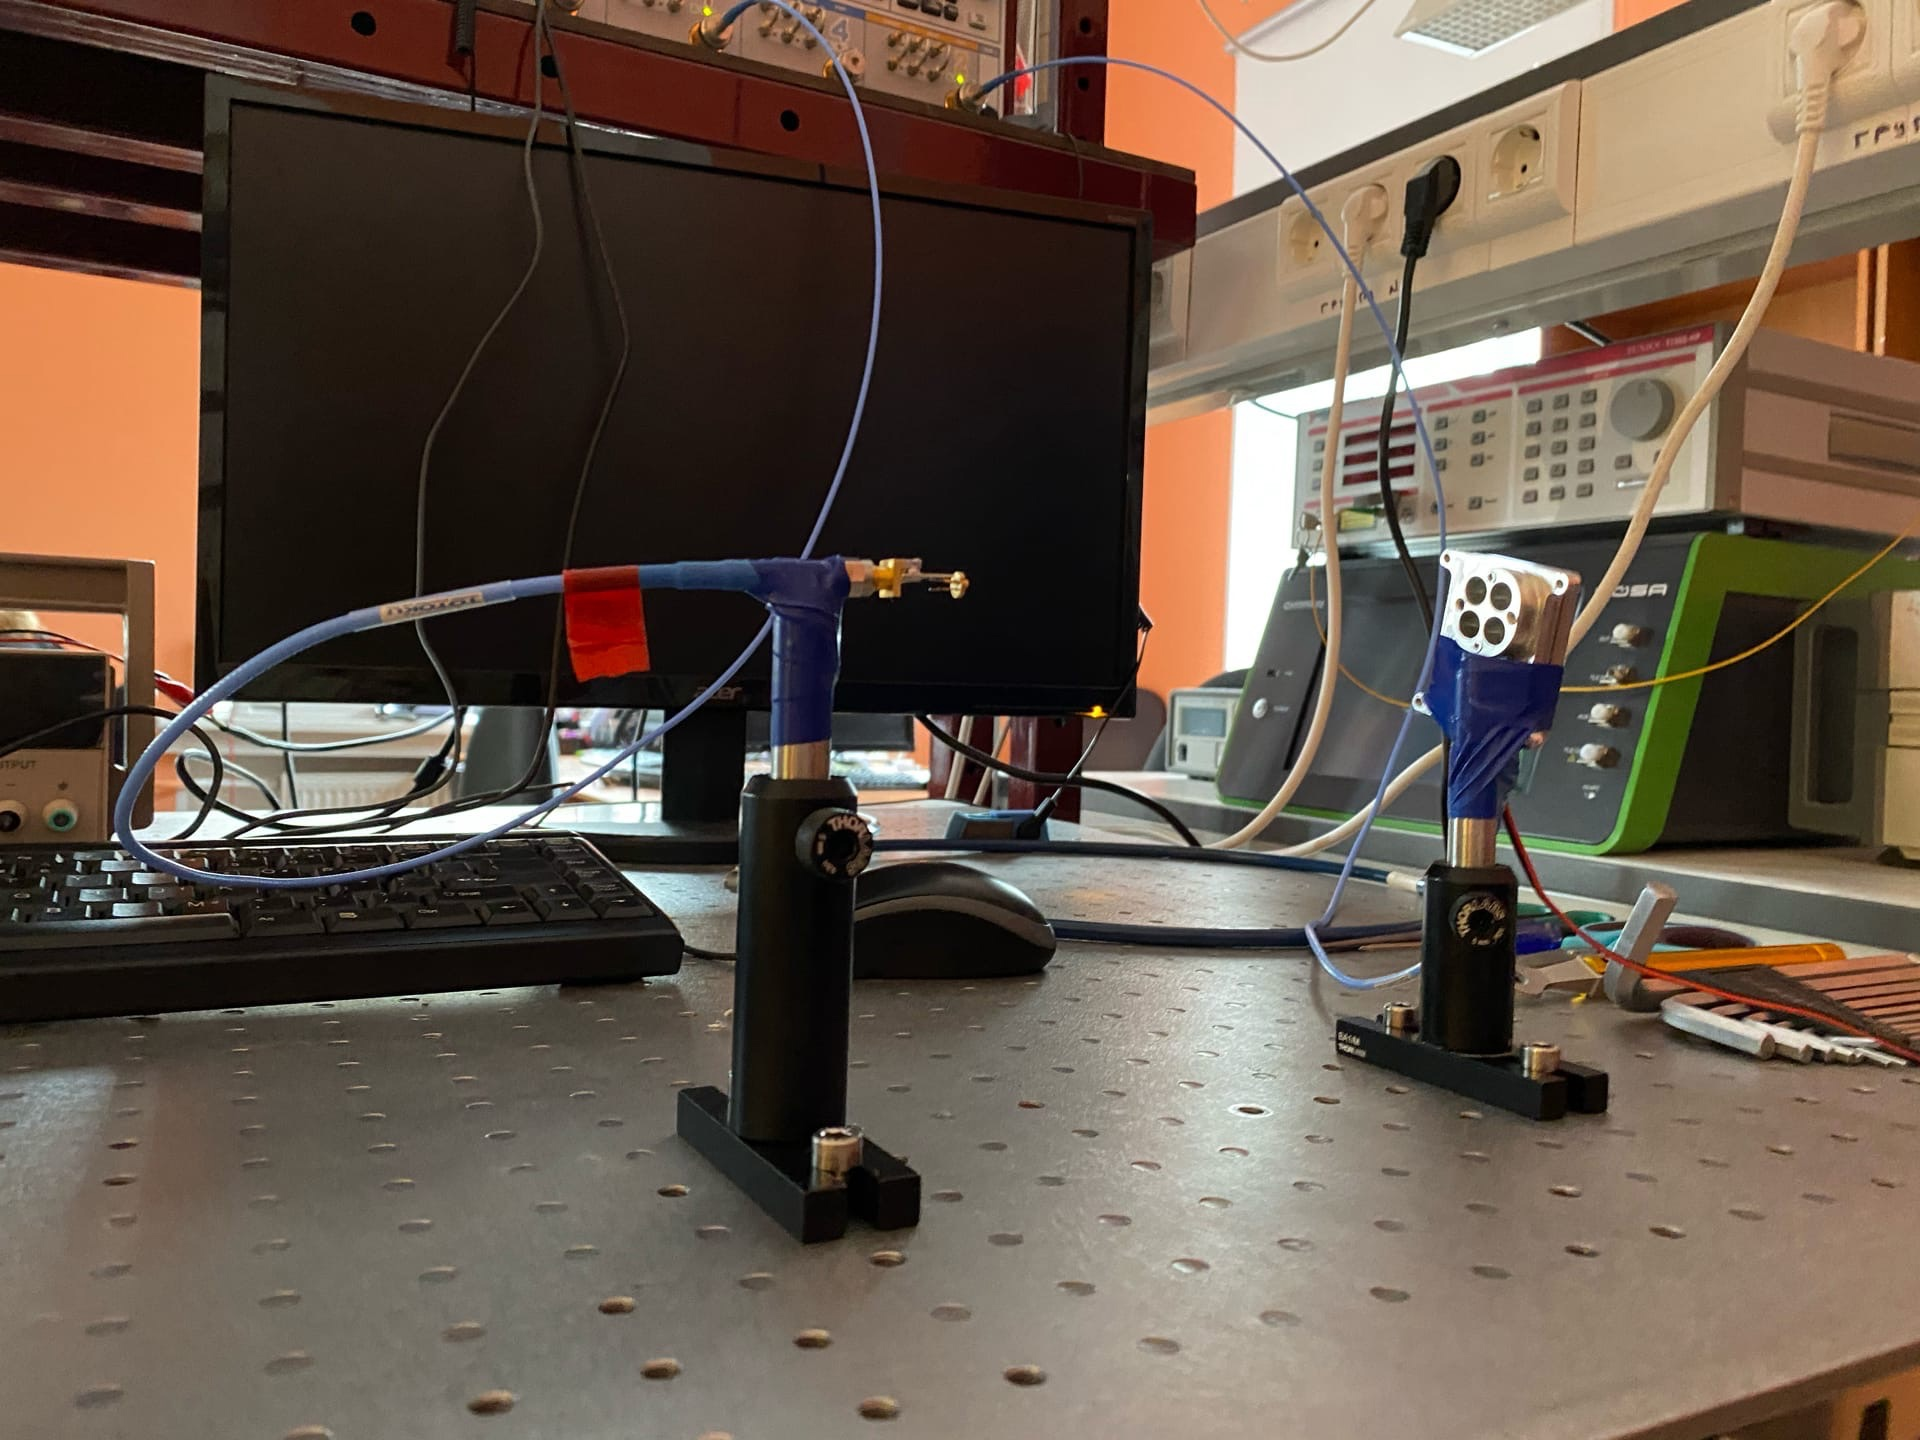
\includegraphics[width=.9\textwidth]{inc/img/experiment_setup.jpg}
    \caption{Собранная экспериментальная установка с лазерным диодом FPL1055T и фотодиодом, использованным в работе~\cite{Kozyreva2019}}
    \label{fig:experiment_setup_photo}
\end{figure}

К первому порту векторного анализатора цепей подключен лазерный диод, ко второму \--- фотодиод. Для расчёта пропускной способности необходимо измерить ёмкость фотодиода экспериментально. Сделаем это при помощи измерения комплексного коэффициента отражения векторным анализатором (полученная диаграмма Смита приведена на рисунке~\ref{fig:smith_plot}).

\begin{figure}[!h]
    \centering
    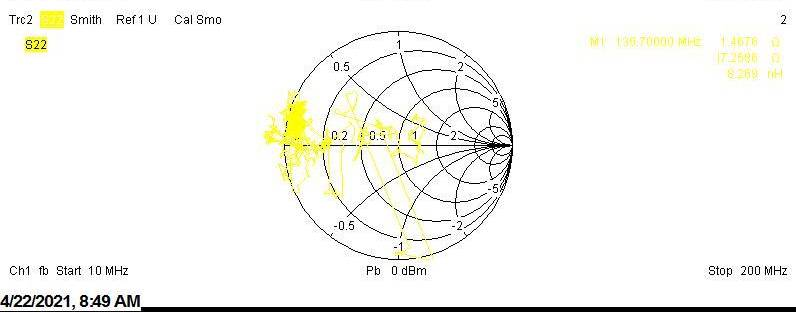
\includegraphics[width=.9\textwidth]{inc/img/smith_plot.jpg}
    \caption{Диаграмма Смита для фотодиода}
    \label{fig:smith_plot}
\end{figure}

По измеренным данным не удаётся демодулировать сигнал из-за большого коэффициента отражения. Это связано с тем, что в сверх высоко частотный тракт ничего не проходит, так как нет согласования фотодиода по высоким частотам. % Для примера, на рисунке приведена диаграмма Смита для фотодиода, использованного в работе~\cite{Kozyreva2019}